\documentclass{standalone}
\usepackage{graphicx}	
\usepackage{amssymb, amsmath}
\usepackage{color}

\usepackage{tikz}
\usetikzlibrary{shapes}
\usepackage{pgfmath}

\definecolor{light}{RGB}{220, 188, 188}
\definecolor{mid}{RGB}{185, 124, 124}
\definecolor{dark}{RGB}{143, 39, 39}
\definecolor{highlight}{RGB}{180, 31, 180}
\definecolor{gray10}{gray}{0.1}
\definecolor{gray20}{gray}{0.2}
\definecolor{gray30}{gray}{0.3}
\definecolor{gray40}{gray}{0.4}
\definecolor{gray60}{gray}{0.6}
\definecolor{gray70}{gray}{0.7}
\definecolor{gray80}{gray}{0.8}
\definecolor{gray90}{gray}{0.9}
\definecolor{gray95}{gray}{0.95}

\newcommand*{\h}{30}

\begin{document}

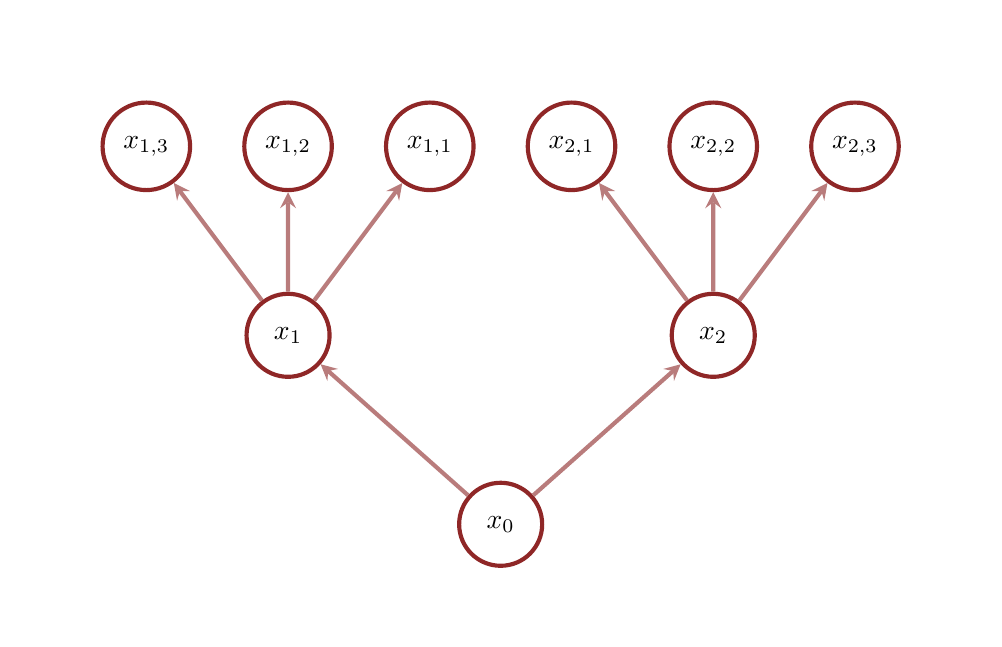
\begin{tikzpicture}[
   scale=0.2,
   obscirc/.style={circle, draw=dark, fill=dark, line width=1.5, text=white,
               inner sep=5, minimum size=\h},
   obsell/.style={ellipse, draw=dark, fill=dark, line width=1.5, text=white,
                  inner sep=5, minimum height=\h, minimum width=50},
   obsrec/.style={rectangle, draw=dark, fill=dark, line width=1.5, text=white,
                  inner sep=5, minimum height=\h, minimum width=\h},
   unobscirc/.style={circle, draw=dark, fill=white, line width=1.5, text=black,
                     inner sep=5, minimum size=\h},
   unobsell/.style={ellipse, draw=dark, fill=white, line width=1.5, text=black,
                    inner sep=5, minimum height=\h}, minimum width=50,
   unobsrec/.style={rectangle, draw=dark, fill=white, line width=1.5, text=black,
                    inner sep=1, minimum height=\h, minimum width=27},
   pushobscirc/.style={circle, draw=white, fill=dark, line width=1.5, dashed, text=white,
                    inner sep=1, minimum size=\h},
   pushunobscirc/.style={circle, draw=dark, fill=white, line width=1.5, dashed, text=black,
                    inner sep=1, minimum size=\h},
   pushell/.style={ellipse, draw=dark, fill=white, line width=1.5, dashed, text=black,
                   inner sep=1, minimum height=\h}
  ]

  % Node Spacing
  \pgfmathsetmacro{\d}{6}
  
  \begin{scope}[shift={(0, 0)}]
    \draw[white] (-5 * \d, -1 * \d) rectangle (5 * \d, 5.25 * \d);

    \node (A) at (0 * \d, 0 * \d) [unobscirc] { $x_{0}$ };
    
    \node (B) at (-2.25 * \d, +2 * \d) [unobscirc] { $x_{1}$ };

    \node (C) at (+2.25 * \d, +2 * \d) [unobscirc] { $x_{2}$ };
    
    \node (D) at (-0.75 * \d, +4 * \d) [unobscirc] { $x_{1, 1}$ };
    \node (E) at (-2.25 * \d, +4 * \d) [unobscirc] { $x_{1, 2}$ };
    \node (F) at (-3.75 * \d, +4 * \d) [unobscirc] { $x_{1, 3}$ };
    
    \node (G) at (+0.75 * \d, +4 * \d) [unobscirc] { $x_{2, 1}$ };
    \node (H) at (+2.25 * \d, +4 * \d) [unobscirc] { $x_{2, 2}$ };
    \node (I) at (+3.75 * \d, +4 * \d) [unobscirc] { $x_{2, 3}$ };
            
    \foreach \B/\E in {A/B, B/D, B/E, B/F, A/C, C/G, C/H, C/I} {
      \draw[->, >=stealth, color=mid, line width=1.5] (\B) -- (\E);
    }

  \end{scope}

\end{tikzpicture}

\end{document}  